Because of the results from the previous test, allowing disimprovement, did not improve the learned preconditioner by any significant degree. Therefore we will go back to looking at the structure of our preconditioner. When initial explaining the structure of the Preconditioner, in section \ref{sec: initial par shift}, in the part about the number of partitions of the superdiagonal. We said that with higher number of partitions could lead to a better preconditioner, but with a longer learning time. Therefore the next test will test for larger amount of partitions and the number of partitions we will test is \(\{15,20,25,30,40,50\}\). To compensate for the potential longer learning time these test will also have an increased base number of learning steps from 100 to 200.

The first thing to notice from the learning curves in figure \ref{fig: more par learning curves}, is that our assumption that having more partitions will equate to longer learning is correct. It can most notable be seen in the test with 50 partition, brown learning curve, as the mean and median solver iteration count does go down but at a slower rate compared to the smaller number of partitions. Starting with a mean solver iteration count of 3086 and decreases it to 2332.3 at learn step 248, but then the solver iteration counts does not change by any substantial amount after that. Compared to the run with 15 partitions gets below a mean solver iteration count 2250 at learn step 138, which means that more partitions have slower learning and it plateaus at higher solver iteration counts.


\begin{figure}[H]
    \center
    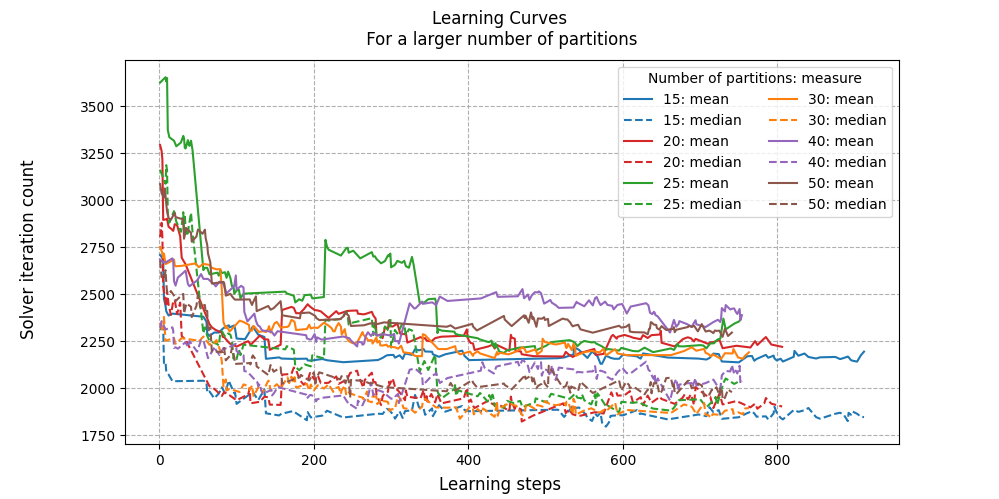
\includegraphics[width=1\textwidth]{plots/more_num_par_learning_curve.png}
    \caption{Learning curves for testing larger number of partitions. Where the colour corresponds to the number of partitions and line style corresponds to mean (whole line) and median (dashed line) solver iteration count.}
    \label{fig: more par learning curves}
\end{figure}

\begin{figure}[H]
    \begin{minipage}{.49\textwidth}
        \center
        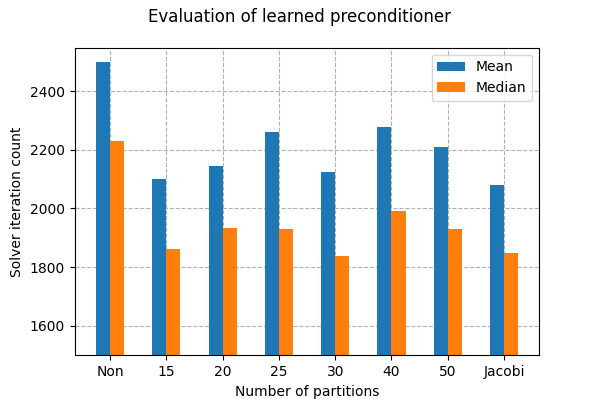
\includegraphics[width=1\textwidth]{plots/more_num_par_test_measure.png}
        \caption{Mean and median solver iteration count indicated by the colour of the bar from the evaluation of the learned preconditioners with different number of partitions indicated by the label.\\\\}
        \label{fig: more par test measure}
    \end{minipage}
    \begin{minipage}{.02\textwidth}
        
    \end{minipage}
    \begin{minipage}{.49\textwidth}
        \center
        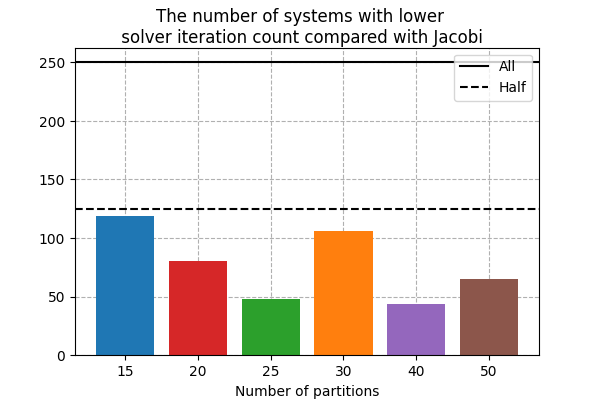
\includegraphics[width=1\textwidth]{plots/more_num_par_BvJ.png}
        \caption{Individual linear system comparison between the learned preconditioners with different number of partitions and Jacobi preconditioners with bar size corresponding to the number of systems where the learned preconditioner has a lower solver iteration count.}
        \label{fig: more par BvJ}
    \end{minipage}
\end{figure}


The second thing is that allowing accepting of worse state makes the learning worse for higher partition counts, as a consequence of the slower learning. It can most notably be seen for the 40 partition count run, purple learning curve. At learn step 324, the mean solver iteration count increases from 2238.3 to 2424.8, and then it does not get below the increase before it the number of learning steps maxed out. Compare this with the run with 25 partitions, which has increase in solver iteration count at learn iteration 215 and does get back to the iteration from before the increase at learn iteration 337. This problem could be improved with a smaller probability for accepting worse states, but then the learning might get stuck in a minimum. 

From the evaluations of the learned Preconditioners, figure \ref{fig: more par test measure} and \ref{fig: more par BvJ}, it is clear that using more partitions does not make the preconditioner better. Even with the change to the algorithm such that it returns the best found preconditioner during learning, as both the mean and median solver iteration count are on par, 15 and 30 partition, or worse than using the Jacobi preconditioning. And for all preconditioners the number of systems that have a lower solver iteration count compared to Jacobi is less than half.